% !Mode:: "TeX:UTF-8"
\chapter{H.265 帧内无损编码 FPGA 原型验证平台}
\label{cha:c5}
当电路系统复杂度高于一定程度时,传统的行为级仿真已经难以满足设计的验证需求,使用 FPGA 进行原型验证灵活度高,验证结果可靠,且有利于软硬件协同设计、加快项目开发进度。因此 FPGA 原型验证成为了复杂系统 ASIC 化之前不可或缺的一个步骤。

\section{FPGA 原型验证方案}
为了对设计的硬件编码器进行验证,本课题设计、搭建了一个完整的 FPGA 原型验证平台。该验证平台由视频源、预处理模块、通信模块、硬件编码器和上位机解码模块组成,利用该平台可实时编码由视频源提供的图像信息,经映射入 FPGA 的硬件编码器编码后将码流传回上位机,在上位机对码流进行网络适配层码流的拼接后,由上位机软解码,实时查看软解码结果正确与否即可对硬件编码器进行验证。完整的验证平台如图 \ref{fig:FPGADemoBlock} 所示。
\begin{figure}[hbt]
    \centering
    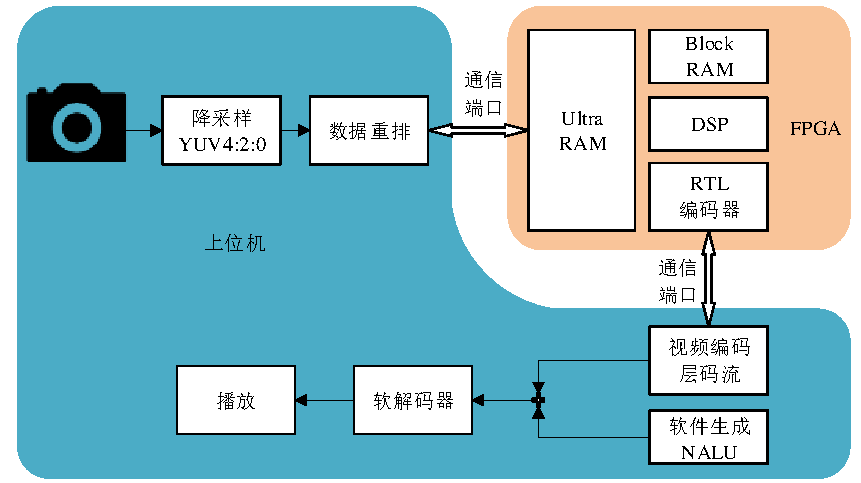
\includegraphics{FPGADemoBlock.pdf}
    \caption{FPGA 原型验证平台}
    \label{fig:FPGADemoBlock}
\end{figure}

\section{验证平台关键模块}
验证平台由上位机与 FPGA 共同组成,上位机进行视频源的获取与预处理,同时负责对 FPGA 输出的码流进行加工、软解码,最终实时播放;FPGA 负责映射硬件编码器,其中使用大量的专用存储器资源实现数据缓存和交换,以保证留出足够的查找表实现编码逻辑的映射。通信端口由上位机和 FPGA 共同处理,根据通信速率的需求可选择串口、以太网口进行通信。
\subsection{FPGA 平台}
\% 简要介绍 FPGA 开发板的可用资源,说明 LUT RAM DSP 等足够映射编码器 \%

\subsection{视频源及预处理}
\% 视频源可用文件、相机、HDMI \%

% 文件 摄像头 显卡HDMI输出
\subsection{与上位机通信接口}
% USB串口CP2102 以太网口 PCIE
\% 通信接口可选 USB转串口、以太网 \%

\subsection{编码模块}
% ultra ram DSP blockram distributionram FIFO
\% 使用 Ultra RAM 与 Block RAM 实现编码器中的大量存储需求 \%

\subsection{上位机解码模块}
% VCL NAL
\% 网络适配层拼接、解码 \%

\section{FPGA 原型验证结果}
% 照片
% 说明摄影环境
与算法软件验证、行为级仿真验证不同,FPGA 原型验证采用编码实时摄像机获取的图像的方式,通过对比硬件编码输出码流的字节数进行验证。验证中选取了室内、走廊、室外和人像 4 个典型场景,验证结果如表 \ref{tab:FPGADemoTestTab} 所示。


验证结果普遍比测试序列优化程度更高,是因为测试序列大多属于较难编码的界面,编码块划分中很少出现大尺寸单元,不利于 L-BPIP 算法的发挥。

\section{本章小结}